\documentclass[10pt]{beamer}

\usepackage{fontspec}
\usepackage{xunicode}
\usepackage{xltxtra}
\setsansfont{FreeSans}
\setmonofont{DejaVuSansMono}

\usepackage{listings}
\usepackage{textpos}
\usepackage{tikz}
\usepackage{minted}

\setbeamertemplate{footline}[frame]
\setbeamertemplate{items}[default]
\usetheme{Warsaw}
\usecolortheme{seahorse}
\setbeamertemplate{itemize items}[default]
\setbeamertemplate{navigation symbols}{}
\setbeamertemplate{footline}[frame number]
\lstset{columns=fixed}
\setbeamerfont*{block body}{series=\tt}
\definecolor{lightgray}{rgb}{0.9,0.9,0.9}
\definecolor{midgray}{rgb}{0.5,0.5,0.5}

\usetikzlibrary{arrows,positioning}
\tikzset{
    %Define standard arrow tip
    >=stealth',
    %Define style for boxes
    actor/.style={
      rectangle,
      rounded corners,
      draw=black, thick,
      text width=4.5em,
      minimum height=1em,
      text centered},
    % Define arrow style
    arr/.style={
      ->,
      thick,
      shorten <=2pt,
      shorten >=2pt,}
}


\newcommand{\light}[1]{\textcolor{gray}{\footnotesize{#1}}}
\newcommand{\code}[4]{\inputminted[linenos, frame=none, firstline=#2, lastline=#3,
  framesep=10pt, bgcolor=lightgray]{#4}{#1}}

\title[Erlang, Haskell, production]{Erlang и Haskell в production: проблемы и решения}
\author{Dmitry Groshev, Fedor Gogolev}
\date{ % \includegraphics[height=3cm]{stadshuset-townhall2}\\
  04.10.2012}
\institute{FProg 2012-10}

% \addtobeamertemplate{frametitle}{}{%
% \begin{textblock*}{100mm}(1\textwidth,-0.7cm)
% \includegraphics[height=0.6cm]{stadshuset-townhall2}
% \end{textblock*}}

\begin{document}
\renewcommand*{\inserttotalframenumber}{\pageref{lastframe}}
\begin{frame}
\titlepage
\end{frame}

\begin{frame}{Общий план}
  \begin{itemize}
  \item Вступление
  \item Коротко о пони
  \item YAWNDB
  \item Selecon-web
  \item Коротко об облаках
  \item Rainbowdash
  \item Twilightsparkle
  \item Резюме
  \end{itemize}
\end{frame}

\begin{frame}
  \begin{center}
    \Large
    Вступление
  \end{center}
\end{frame}

\begin{frame}{Вступление}
  \begin{itemize}
  \item 1.5 года production-experience с Erlang
  \item 1 год с Haskell
  \item In-memory timeseries database (YAWNDB)
  \item Система нотификации (Spike)
  \item Веб-консоль (Selecon-web)
  \item Облако (Rainbowdash/Twilightsparkle)
  \end{itemize}
\end{frame}

\begin{frame}
  \begin{center}
    \Large
    Коротко о пони
  \end{center}
\end{frame}

\begin{frame}[plain]
  \begin{tikzpicture}[remember picture,overlay]
    \node[at=(current page.center)] {
      
\includegraphics[height=\paperheight]{ponies.jpg}
    };
  \end{tikzpicture}
\end{frame}

\begin{frame}
  \begin{center}
    \Large
    YAWNDB
  \end{center}
\end{frame}

\begin{frame}{YAWNDB}
  \begin{itemize}
  \item Timeseries данные
  \item Много операций записи (десятки тысяч в секунду)
  \item Хочется аггрегацию
  \item Graphite медленный, RRD не умеет аггрегацию
  \end{itemize}
  Yet Another Weel iNvented
\end{frame}

\begin{frame}{YAWNDB}
  \begin{tikzpicture}[node distance=1cm, auto,]
    \node[] (col1) {};
    \node[right=2.5cm of col1] (col2) {};
    \node[right=2.5cm of col2] (col3) {};
    \node[right=2.5cm of col3] (col4) {};

    \node[actor, below=2cm of col1] (req1) {request handler 1};
    \node[actor, below=0.5cm of req1] (req2) {request handler 2};
    \node[actor, below=0.5cm of req2] (req_more) {...};
    \node[actor, below=0.5cm of req_more] (reqn) {request handler N};

    \node[actor, below=0.5cm of col2] (pathmgr) {Path manager}
    edge[arr, <-, bend right=20] node[auto, font=\footnotesize]
      {New path} (req1);

    \node[actor, below=2cm of col3] (path1) {path 1}
    edge[arr, <-, bend right=25] (pathmgr)
    edge[arr, <-, bend left=10] (req1.east);
    \node[actor, below=0.5cm of path1] (path2) {path 2}
    edge[arr, <-, bend right=10] (req2.east);
    \node[actor, below=0.5cm of path2] (path3) {path 3}
    edge[arr, <-, bend left=10] (req2.east);
    \node[actor, below=0.5cm of path3] (path_more) {...};
    \node[actor, below=0.5cm of path_more] (pathm) {path M};

    \node[actor, below=0.5cm of col4, sharp corners] (disk) {Disk};
    \node[actor, below=1.5cm of disk] (dumper) {Dumper}
    edge[arr, ->] (disk)
    edge[arr, <->, bend left=10] (path1.east)
    edge[arr, <->, bend right=10] (path2.east)
    edge[arr, <->, bend left=10] (path3.east)
    edge[arr, <->, bend left=10] (pathm.east);
  \end{tikzpicture}
\end{frame}

\begin{frame}{YAWNDB: выводы}
  \begin{itemize}
  \item NIF это круто, но опасно
  \item мутабельные NIF binaries предоставляют изолированную мутабельность
  \item писать NIF неприятно, документация полна, но не всегда
    помогает
  \item property-based тестирование при использовании NIF необходимо,
    т.к. ошибки нетривиальны, а segfault'ы травматичны
  \item fuzz-тесты на случайных/бессмысленных данных полезны
  \item писать высококонкурентные системы сложно, Erlang не добавляет
    сложности
  \item устойчивость к ошибкам Erlang'а помогает, в продакшне почти
    полгода был редкий рейс без последствий вообще
  \end{itemize}
\end{frame}

\begin{frame}{YAWNDB: выводы 2}
  \begin{itemize}
  \item код лаконичен (650 строк на C, 1500 строк на Erlang'е)
  \item если вы пишите что-то сетевое, нет ни одной причины не
    использовать Cowboy
  \item поддержка SMP Erlang'ом не миф
  \end{itemize}
  \begin{center}
    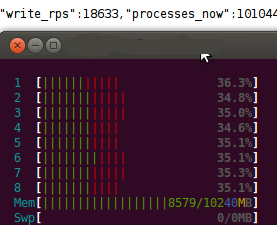
\includegraphics[width=.5\textwidth]{top.png}
  \end{center}
\end{frame}

\begin{frame}{YAWNDB: ссылки}
  \begin{itemize}
  \item Ecirca \url{https://github.com/band115/ecirca}
  \item Cowboy \url{https://github.com/extend/cowboy}
  \item McErlang \url{https://github.com/fredlund/McErlang}
  \end{itemize}
\end{frame}

\begin{frame}
  \begin{center}
    \Large
    Облака
  \end{center}
\end{frame}

\begin{frame}{Об облаках}
  Xen:
  \begin{itemize}
  \item Dom0, DomU
  \item запуск и остановка доменов
  \item простой и неубиваемый
  \end{itemize}
  XAPI (XenAPI) от Citrix:
  \begin{itemize}
  \item Миграция
  \item Пулы
  \item Драйвера устройств
  \item Динамическое управление памятью
  \item ...
  \end{itemize}
\end{frame}

\begin{frame}[plain]
  \begin{tikzpicture}[remember picture,overlay]
    \node[at=(current page.center)] {
      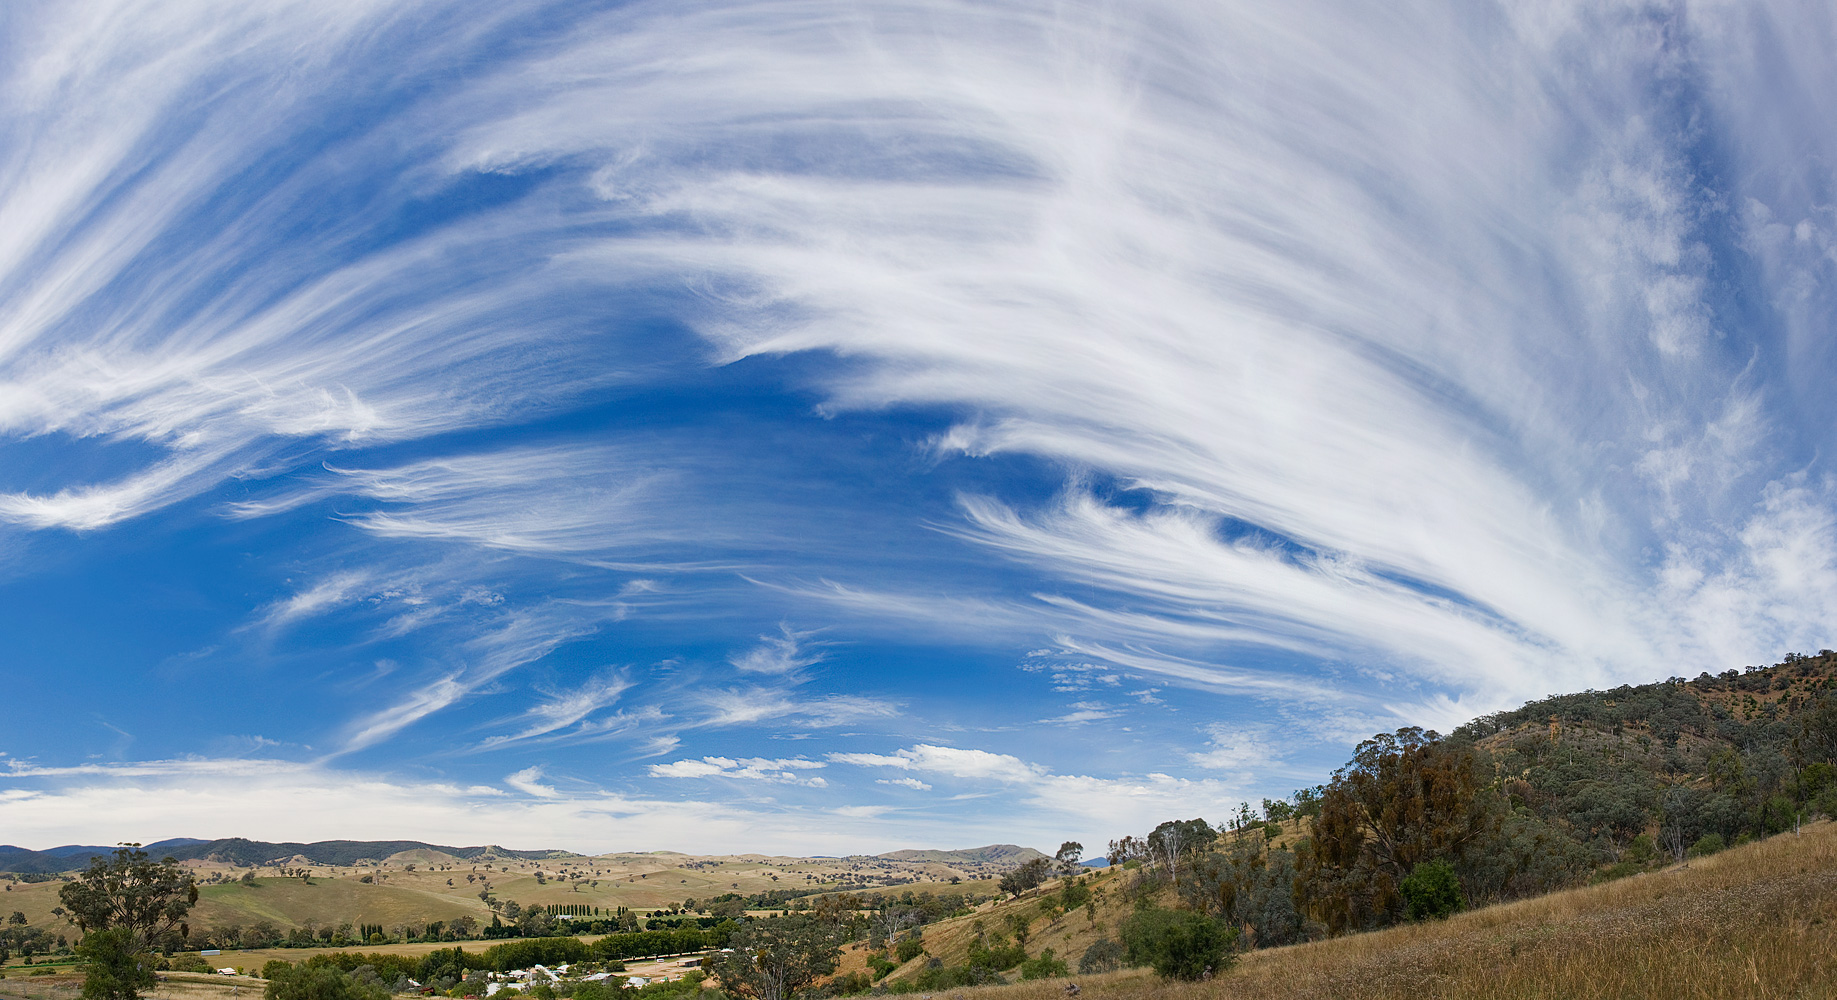
\includegraphics[height=\paperheight]{clouds.jpg}
    };
  \end{tikzpicture}
\end{frame}

\begin{frame}{Haskell test}
  \begin{center}
    \footnotesize
    \code{code.hs}{1}{12}{haskell}
  \end{center}
\end{frame}

\begin{frame}\label{lastframe}
  Copyrighted stuff:
  https://en.wikipedia.org/wiki/File:Cirrus\_sky\_panorama.jpg \\
  http://www.wallpapervortex.com/wallpaper-15684\_1\_other\_wallpapers\_my\_little\_pony.html
\end{frame}